\documentclass[11pt]{article}
\usepackage[spanish, activeacute]{babel}
\usepackage[latin1]{inputenc}
\usepackage{amsmath, amssymb}
\usepackage{graphicx}
\usepackage{anysize}
\usepackage[a4paper=true]{hyperref}
\usepackage{caption}    
\title{Presencia del Observatorio Virtual en el Mundo}
\author{Jos\'{e} David Marroqu\'{i}n Toledo}
\date{13th of April, 2013}
\marginsize{3cm}{2cm}{0.5cm}{3cm}

\begin{document}
     \begin{center}
         \huge{\textbf{Presencia del Observatorio Virtual en el Mundo}}
     \end{center}
     \begin{center}
         \large{Jos\'{e} David Marroqu\'{i}n Toledo}

         \small{Universidad T\'{e}cnica Federico Santa Mar\'{i}a}
     \end{center}

     \section{Resumen}
         Este documento da a conocer los proyectos de observatorios virtuales
que conforman la Alianza Internacional Observatorio Virtual (IVOA por sus siglas
en ingl\'{e}s), c\'{o}mo est\'{a}n distribuidos en todo el mundo y a trav\'{e}s
de una breve descripci\'{o}n, las herramientas que ellos mismos desarrollan bajo
est\'{a}ndares que facilitan el compartimiento del conocimiento astron\'{o}mico
y la interoperabilidad. Para esta investigaci\'{o}n fueron revisados el sitio
\textit{web} de IVOA y los de sus miembros, publicaciones cient\'{i}ficas,
art\'{i}culos en libros y otras fuentes electr\'{o}nicas. Este documento es
requerido por una iniciativa que pretende desde Chile el desarrollo de una
plataforma astro-inform\'{a}tica para administrar y analizar inteligentemente
datos a gran escala basados en los est\'{a}ndares de IVOA, proyecto que
involucra la participaci\'{o}n activa de estudiantes de la Universidad
T\'{e}cnica Federico Santa Mar\'{i}a.

     \section{Introducci\'{o}n}
         El Observatorio Virtual (VO por sus siglas en ingl\'{e}s) es una
iniciativa internacional que permite el acceso a archivos astron\'{o}micos y
centros de datos a astr\'{o}nomos y personas comunes a trav\'{e}s de Internet.
Con la estandarizaci\'{o}n de m\'{e}todos e informaci\'{o}n es posible estudiar
los registros astron\'{o}micos sin requerimientos f\'{i}sicos de instrumentos y
locaci\'{o}n.\\

         En junio de 2002, fue creada la Alianza Internacional Observatorio
Virtual para ``facilitar la coordinaci\'{o}n internacional y colaboraci\'{o}n
necesaria para el desarrollo y distribuci\'{o}n de herramientas, sistemas y
estructuras organizacionales necesarias para permitir la utilizaci\'{o}n
internacional de archivos astron\'{o}micos como un observatorio virtual
integrado e interoperable\footnote{Traducido de
\url{http://www.ivoa.net/about/what-is-ivoa.html} el mi\'{e}rcoles, 15 de mayo
de 2013 por Jos\'{e} D. Marroqu\'{i}n Toledo}. Actualmente, IVOA est\'{a}
compuesta por 19\footnote{En el sitio web oficial en la secci\'{o}n
\textbf{Whats is the IVOA} \textit{``the IVOA now comprises 17 VO projects''},
pero en \textbf{Members Organizations} aparecen 19 miembros listados.} proyectos
de Am\'{e}rica, Asia, Europa y Ocean\'{i}a; sus miembros se reunen dos veces
cada a\~{n}o en \textbf{Interoperability Workshops} para entablar discusiones
cara-a-cara y resolver preguntas t\'{e}cnicas.\\

         Una iniciativa liderada por el Dr. Mauricio Solar junto a estudiantes
de la Universidad T\'{e}cnica Federico Santa Mar\'{i}a pretende desarrollar una
plataforma astro-inform\'{a}tica para la administraci\'{o}n y an\'{a}lisis
inteligente de datos a gran escala basados en los est\'{a}ndares de IVOA. Por lo
anterior, este documento tiene como objetivo:

         \begin{itemize}
             \item Dar a conocer la distribuci\'{o}n de los observatorios
virtuales en el mundo.
             \item Listar las herramientas desarrolladas por los observatorios
virtuales y sus estados desde la informaci\'{o}n provista en sus sitios web
oficiales en Internet.
             \item Dar una idea acerca de qu\'{e} herramientas adicionales
podr\'{i}an ser desarrolladas para garantizar el complimiento del objetivo
principal\footnote{\textit{``Desarrollo de una plataforma astro-inform\'{a}tica
para la administraci\'{o}n y an\'{a}lisis inteligente de datos a gran escala''}
acorde al nombre del proyecto Fondef D11$ \vert $1060.}
         \end{itemize}

         Para estos prop\'{o}sitos fueron revisados el sitio \textit{webs}
oficial de la IVOA y los de sus miembros, le\'{i}das secciones de documentos
acerca de observatorios virtuales como ``Virtual Observatories, Data Mining, and
Astroinformatics''de Kirk Borne, George Mason University, entre otros.\\

     \section{Distribuci\'{o}n de los observatorios virtuales en el mundo}
         \subsection{IVOA}
             Desde el a\~{n}o 2002, proyectos de observatorios virtuales
comenzaron a integrar la Alianza Internacional Observatorio Virtual (IVOA) bajo
el \textbf{Guidelines for Participation\footnote{Lineamientos disponibles en un
\textit{paper} en formatos PDF y DOC en
\url{http://www.ivoa.net/documents/latest/IVOAParticipation.html}}}. Estos
fueron fundados bajo programas privados y gubernamentales nacionales e
internacionales en colaboraci\'{o}n con centro de estudios cient\'{i}ficos,
universidades y otros. Quienes integran este proyecto, el Observatorio Virtual
(VO por sus siglas en ingl\'{e}s), comparten conocimientos entre ellos y la
comunidad de modo estandarizado. Son ellos mismos quienes desarrollan estos
est\'{a}ndares para el intercambio de informaci\'{o}m e interoperabilidad.\\
            
             La tabla 1 muestra los socios de IVOA hasta mayo de
2013\footnote{En este documento, toda la informaci\'{o}n recuperada del sitio
\textit{web} oficial de IVOA es considerada oficial y ver\'{i}dica.}.

             \begin{center}
                 \begin{tabular}{|p{7cm} | p{7cm}|}
                     \hline
                     \textbf{Proyecto} & \textbf{URL} \\
                     \hline
                     Argentina Virtual Observatory &
\url{http://nova.conicet.gov.ar/} \\
                     \hline
                     Armenian Virtual Observatory &
\url{http://www.aras.am/Arvo/arvo.htm} \\
                     \hline
                     AstroGrid & \url{http://www.astrogrid.org/} \\
                     \hline
                     Australian Virtual Observatory &
\url{http://aus-vo.org.au/} \\
                     \hline
                     Brazilian Virtual Observatory &
\url{http://www.lna.br/bravo/} \\
                     \hline
                     Canadian Virtual Observatory &
\url{http://www.china-vo.org/} \\
                     \hline
                     Chinese Virtual Observatory &
\url{http://www.cadc-ccda.hia-iha.nrc-cnrc.gc.ca/cvo/} \\
                     \hline
                     European Space Agency &
\url{http://www.sciops.esa.int/index.php?project=ESAVO} \\
                     \hline
                     European Virtual Observatory &
\url{http://www.euro-vo.org/} \\
                     \hline
                     German Astrophysical Virtual Observatory &
\url{http://www.g-vo.org/} \\
                     \hline
                     Hungarian Virtual Observatory &
\url{http://hvo.elte.hu/en/} \\
                     \hline
                     Italian Virtual Observatory & \url{http://vobs.astro.it/}
\\
                     \hline
                     Japanese Virtual Observatory & \url{http://jvo.nao.ac.jp/}
\\
                     \hline
                     Observatorie Virtual France &
\url{http://www.france-vo.org/} \\
                     \hline
                     Russian Virtual Observatory &
\url{http://www.inasan.rssi.ru/eng/rvo/} \\
                     \hline
                     Spanish Virtual Observatory &
\url{http://svo.cab.inta-csic.es/} \\
                     \hline
                     Ukranian Virtual Observatory & \url{http://www.ukr-vo.org/}
\\
                     \hline
                     Virtual Astronomical Observatory &
\url{http://www.usvao.org/} \\
                     \hline
                     Virtual Observatory India &
\url{http://vo.iucaa.ernet.in/~voi/} \\
                     \hline
                 \end{tabular}
        
             Table 1. Socios de IVOA.
             \end{center}

             Almost half of IVOA virtual observatories are supported in Europa:
9 of the total; 1 belong to Oceania, 4 to America and 5 of them to
Asia\footnote{As the mayor part of Rusia's territory is in Asia, it was
considered in the virtual observatories of this continent.}. The figure 1 shows
the distribution of the membership per continent.\\

             \begin{figure}[h]
                  \begin{center}
                      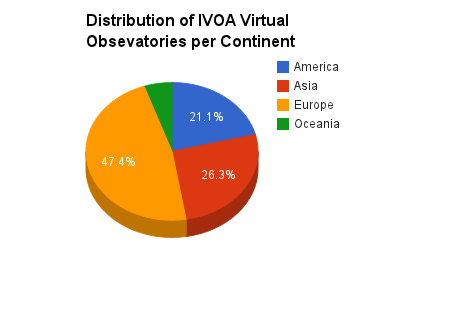
\includegraphics[width=110mm]
{IVOA_VOs_distribution_per_continent_by_JDMT.png}
                      \caption{International Virtual Observatory Alliance
distribution per continent.}
                  \end{center}
             \end{figure}
            
             If Chile became part of International Virtual Observatory Alliance,
the distribution of the members per continent will be as shown in the figure
2.\\

             \begin{figure}[h]
                 \begin{center}
                     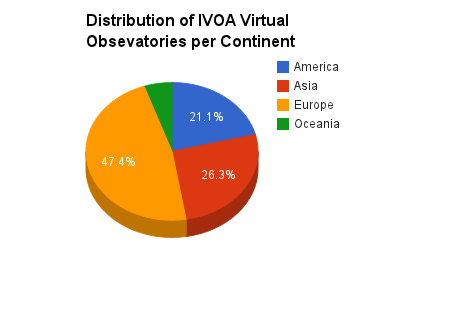
\includegraphics[width=110mm]
{IVOA_VOs_distribution_per_continent_by_JDMT.png}
                     \caption{International Virtual Observatory Alliance
distribution per continent.}
                 \end{center}
             \end{figure}

             Whithout considering the status of the internal projects of the
virtual observatories, the memberships of Chile would contribute to the
cooperation, development and interoperability in the same was as the Asia.
Furthermore, this fact would be very significant, because a large numbers of
astronomical centers like observatories are placed in this country. For now, is
intended to work with a certain quantity of data of ALMA.\\

     \section{Lista of los observatorios virtuales de IVOA y sus proyectos}
         \subsection{America}
              \subsubsection{Brazilian Virtual Observatory (BRAVO)}
                  \begin{itemize}
                      \item Launching: 18th of August, 2008
                      \item Projects
                         \begin{itemize}
                             \item BRAVO@IAG
                             \item BRAVO@INPE
                                  \begin{itemize}
                                      \item Description: generate investment in
information technology on Computational Infraestructure, Date Grid, Data
Processing and Data Mining.
                                      \end{itemize}
                             \item BRAVO@LNA
                                  \begin{itemize}
                                      \item Description: Making of a virtual
observatory dedicated to Southern Astrophysical Research Telescope (SOAR) data
from Brazilian astronomers.
                                  \end{itemize}
                             \item BRAVO@UFSC
                                  \begin{itemize}
                                      \item Description: researching of the of
the power spectral synthesis as a mean to estimate the physical properties of
the galaxies.
                                  \end{itemize}
                             \item CYCLOPS
                         \end{itemize}
                  \end{itemize}

              \subsubsection{Canadian Virtual Observatory (CVO)}
                  \begin{itemize}
                      \item Projects
                          \begin{itemize}
                              \item Data Sharing (VOSpace 2.0)
                                  \begin{itemize}
                                      \item Description: a service which allows
users to share files and collaborate with team members.  
                                  \end{itemize}
                              \item Table Access Protocol (TAP-1.0)
                                  \begin{itemize}
                                      \item Description: a service which allows
the access to all the data described by the Common Archive Observation Model
(CAOM) in use at the CADC and tables from other projects.
                                  \end{itemize}
                              \item Observation Model Core Components
(ObsCore-1.0)
                                  \begin{itemize}
                                      \item Description: a model which
implements a standard view for \textbf{Table Access Protocol (TAP-1.0)}.
                                  \end{itemize}
                              \item Simple Image Access (SIA-1.0)
                                  \begin{itemize}
                                      \item Description: a SIA-1.0 compliant
query service for easy access to calibrated images from most our data
collections.
                                  \end{itemize}
                          \end{itemize}
                  \end{itemize}

             \subsubsection{Nuevo Observatorio Virtual Argentino (NOVA)}
                 \begin{itemize}
                     \item Founders: Observatorio Astron\'{o}mico de C\'{o}rdova
(OAC), Facultad de Ciencias Astron\'{o}micas y Geof\'{i}sicas de La
Plata/Universidad de Nacional de la Plata (FCAGLP/UNLP), Instituto de
Astrof\'{i}sica de La Plata (IALP), Instituto Argentino de Radioastronom\'{i}a
(IAR), Instituto de Astronom\'{i}a y F\'{i}sica del Espacio (IAFE), Instituto de
Ciencias Astron\'{o}micas, de la Tierra y del Espacio (ICAFE), Instituto de
Astronom\'{i}a Te\'{o}rica y Experimental (IATE), Complejo Astron\'{o}mico El
Leoncito (CASLEO).
                     \item Launching: January, 2009
                     \item Projects
                          \begin{itemize}
                              \item NOVA@CASLEO
                                  \begin{itemize}
                                      \item Status: active.
                                      \item Description: not obtained for now.
Not available at NOVA's website or similar.
                                  \end{itemize}
                              \item NOVA@IAFE
                                  \begin{itemize}
                                      \item Status: unknown.
                                      \item Description: building a database for
the spectroscopic observations available at ICATE.
                                      \item Outstanding: until 1987, the
database was stored in photographic plates. After that
year, the information was stored in CDs and DVDs.
                                  \end{itemize}
                              \item NOVA@ICATE
                                  \begin{itemize}
                                      \item Status: unknown.
                                      \item Description: building a database for
the spectroscopic observations available at ICATE.
                                      \item Outstanding: until 1987, the
database was stored in photographic plates.  After that year, the information
was stored in CDs and DVDs.
                                  \end{itemize}
                              \item NOVA@OAC
                                  \begin{itemize}
                                      \item Status: active.
                                      \item Description: not obtained for now.
Not available at NOVA's website or similar.
                                  \end{itemize}
                              \item NOVA@FCAGLP, NOVA@IALP, NOVA@IAR, NOVA@IATE
are referred in the website but without status and description.
                          \end{itemize}
                 \end{itemize}

             \subsubsection{US Virtual Astronomical Observatory (VAO)}
                  \begin{itemize}
                      \item Founders: NSF, NASA.
                      \item Projects
                          \begin{itemize}
                              \item Data Discovery Tool
                                  \begin{itemize}
                                      \item Description: 
                                  \end{itemize}
                              \item Iris: SED Analysis Tool
                                  \begin{itemize}
                                      \item Description: 
                                  \end{itemize}
                              \item Cross-Comparision Tool
                                  \begin{itemize}
                                      \item Description: 
                                  \end{itemize}
                              \item Time Series Search Tool
                                  \begin{itemize}
                                      \item Description: 
                                  \end{itemize}
                          \end{itemize}
                  \end{itemize}

          \subsection{Europe}
              \subsubsection{Armenian Virtual Observatory}
                  \begin{itemize}
                      \item Projects
                  \end{itemize}

              \subsubsection{Hungarian Virtual Observatory (HVO)}
                  \begin{itemize}
                      \item Projects
                  \end{itemize}

              \subsubsection{AstroGrid}
                  \begin{itemize}
                      \item Launching: 2001
                      \item Founders: PPARC, STFC
                      \item Projects
                          \begin{itemize}
                              \item VODesktop
                                  \begin{itemize}
                                      \item Description: an analysis tools wich
allows limit the choice of resources through specific data saving.
                                  \end{itemize}
                              \item Astro Runtime (AR)
                                  \begin{itemize}
                                      \item Description: an API implemented in
JAVA wich facilitates the access to the \textbf{VODesktop} services from any
programming language.
                                  \end{itemize}
                          \end{itemize}
                  \end{itemize}

              \subsubsection{European Space Agency Virtual Observatory (ESA-VO)}
                  \begin{itemize}
                      \item Projects
                  \end{itemize}

              \subsubsection{European Virtual Observatory (EURO-VO)}
                  \begin{itemize}
                      \item
                  \end{itemize}

              \subsubsection{German Astrophysical Virtual Observatory (GAVO)}
                  \begin{itemize}
                      \item Projects
                          \begin{itemize}
                              \item GAVO Data Center
                                  \begin{itemize}
                                      \item Description: A growing collection of
data and services provided on behalf of third parties. Some of the GAVO services
are also available on http://dc.zah.uni-heidelberg.de/
                                  \end{itemize}
                              \item MPA Simulations access
                                  \begin{itemize}
                                      \item Description: a web service for
querying the results of the Millennium simulation using SQL.
                                  \end{itemize}
                              \item MultiDark Database
                                  \begin{itemize}
                                      \item Description: a service wich gives
access to data from MultiDark and Bolshoi simulations using SQL queries. It
based on the Millennium Web Application.
                                  \end{itemize}
                              \item RAVE archive search
                                  \begin{itemize}
                                      \item Description: an access to a growing
archive of radial velocities for more than 400 000 stars.
                                  \end{itemize}
                              \item TheoSSA
                                  \begin{itemize} \item Description: a service
for providing spectral energy distributions based on model atmosphere
calculations.
                                  \end{itemize}
                          \end{itemize}
                  \end{itemize}

              \subsubsection{Observatoire Virtuel France (VO-France)}
                  \begin{itemize}
                      \item Projects
                  \end{itemize}

              \subsubsection{Spanish Virtual Observatory (SVO)}
                  \begin{itemize}
                      \item Projects
                          \begin{itemize}
                              \item VOSA
                                  \begin{itemize}
                                      \item Description: 
                                  \end{itemize}
                              \item VOSED
                                  \begin{itemize}
                                      \item Description: 
                                  \end{itemize}
                              \item TESELA
                                  \begin{itemize}
                                      \item Description: 
                                  \end{itemize}
                              \item Filter Profile Service
                                  \begin{itemize}
                                      \item Description: 
                                  \end{itemize}
                          \end{itemize}
                  \end{itemize}

              \subsubsection{Italian Virtual Observatory (VObs.it)}
                  \begin{itemize}
                      \item Launching: 2005
                      \item Founders: INAF
                      \item Projects
                          \begin{itemize}
                              \item SIAP
                                  \begin{itemize}
                                      \item Description: 
                                  \end{itemize}
                              \item SSAP
                                  \begin{itemize}
                                      \item Description: 
                                  \end{itemize}
                              \item CONE SEARCH
                                  \begin{itemize}
                                      \item Description: 
                                  \end{itemize}
                              \item SKYNODE
                                  \begin{itemize}
                                      \item Description: 
                                  \end{itemize}
                          \end{itemize}
                  \end{itemize}

      \subsection{Asia}
          \subsubsection{Chinese Virtual Observatory}
              \begin{itemize}
                  \item Projects
              \end{itemize}

          \subsubsection{Japanese Virtual Observatory}
              \begin{itemize}
                  \item Projects
              \end{itemize}

          \subsubsection{Russian Virtual Observatory}
              \begin{itemize}
                  \item Projects
              \end{itemize}

          \subsubsection{Virtual Observatory India}
              \begin{itemize}
                  \item Founders: Persistent Systems Ltd.
                  \item Collaborator: Inter-University Centre for Astronomy and
Astrophysics (IUCAA).
                  \item Supporter: Ministry of Communication and Information
Technology, Government of India.
                  \item Launching: January, 2009
                  \item Projects
                      \begin{itemize}
                          \item VOIPortal
                          \item Mosaic Service
                          \item PyMorph Service
                          \item VOPlot
                          \item VOMegaPlot (Client-Server Version)
                          \item AstroStat
                          \item VOCat
                          \item VOPlatform
                          \item VOConvert (ConVOT)
                          \item Android Cosmological Calculator
                          \item Android Name Resolver
                          \item CSharpFITS Package
                          \item VOTable JAVA Streaming Writer
                          \item C++ parser for VOTable
                          \item Fits Manager
                          \item HCT Data Archival Sys
                      \end{itemize}   
              \end{itemize}

      \section{Conclusiones y recomendaciones}

      \newpage

      \section{Referencias}
          Hanisch, R., \& Quinn, P. (s.f.) The International Virtual
Observatory. Recuperado de \url{http://www.ivoa.net/about/TheIVOA.pdf}\\

          Borne, K. (s.f.) Virtual Observatories, Data Mining, and
Astroinformatics. In H.E. Bond (Ed.), \textit{Planets, Stars and Stellar
Systems} (pp. 409-443). Vol. 2. Dordrecht: Springer Science$ + $Business
Media.\\

          Anonymous. (17 de abril de 2013). Proyecto Fondef: Innovador proyecto
de la USM proveer\'{a} a la Red de Telescopios ALMA de un sofisticado
observatorio virtual. Recuperado de
\url{http://www.conicyt.cl/fondef/2013/04/17/proyecto-fondef-innovador-proyecto-de-la-usm-proveera-a-la-red-de-telescopios-alma-de-un-sofisticado-observatorio-virtual/}\\

          FONCEA, V. (12 de abril de 2013). Observatorios Virtuales: Desarrollo
chileno de astroinform\'{a}tica para ALMA. Recuperado de
\url{http://www.almaobservatory.org/es/anuncios-eventos/542-virtual-observatories-chilean-development-of-astronomical-computing-for-alma}\\

\end{document}
